%%%%%%%%%%%%%%%%%%%%%%%%%%%%%%%%%%%%%%%%%%%%%%%%%%%%%%%
%%% 美国大学生数学建模竞赛(MCM/ICM)论文模板
%%% 来源网站:www.latexstudio.net
%%% 中文注释:小嗷犬 blog.marquis.eu.org
%%%%%%%%%%%%%%%%%%%%%%%%%%%%%%%%%%%%%%%%%%%%%%%%%%%%%%%
%%% code: 代码文件夹
%%% figures: 图片文件夹
%%% *.cls: LaTeX 格式文件
%%% *.tex: LaTeX 文档文件
%%% *.bib: Bib 引用文献源文件
%%%%%%%%%%%%%%%%%%%%%%%%%%%%%%%%%%%%%%%%%%%%%%%%%%%%%%%

%%%%%%%%%%%%%%%%%%%%%%%%%%%%%%%%%%%%%%%%%%%%%%%%%%%%%%%
%%% 可能用到的网站
%%%%%%%%%%%%%%%%%%%%%%%%%%%%%%%%%%%%%%%%%%%%%%%%%%%%%%%
%%% LaTeX公式编辑器:https://www.latexlive.com/
%%% Diagram流程图绘制:https://www.drawio.com/
%%%%%%%%%%%%%%%%%%%%%%%%%%%%%%%%%%%%%%%%%%%%%%%%%%%%%%%

%%%%%%%%%%%%%%%%%%%%%%%%%%%%%%%%%%%%%%%%%%%%%%%%%%%%%%%
%%% 模板参数设置
%%%%%%%%%%%%%%%%%%%%%%%%%%%%%%%%%%%%%%%%%%%%%%%%%%%%%%%
\documentclass{mcmthesis}  % 文档类型
\mcmsetup{CTeX = false,   % 使用 CTeX 套装时,设置为 true
        tcn = 12345678,   % 队伍控制号
        problem = B,  % 选题
        sheet = true,   % sheet页
        titleinsheet = true,   % sheet页显示标题
        keywordsinsheet = true,  % sheet页显示关键词
        titlepage = false,   % 标题页
        abstract = true  % 摘要
        }
%%%%%%%%%%%%%%%%%%%%%%%%%%%%%%%%%%%%%%%%%%%%%%%%%%%%%%%

%%%%%%%%%%%%%%%%%%%%%%%%%%%%%%%%%%%%%%%%%%%%%%%%%%%%%%%
%%% 导入宏包和引用文献源
%%%%%%%%%%%%%%%%%%%%%%%%%%%%%%%%%%%%%%%%%%%%%%%%%%%%%%%
\usepackage{longtable}
\usepackage{float}
\usepackage{graphicx}
\usepackage{indentfirst}%首行缩进
\setlength{\parindent}{2em}
\usepackage{palatino}  % 帕拉提诺体字体宏包
\usepackage{lipsum}  % 导入生成段落的宏包
\usepackage[hyperref=true,style=ieee]{biblatex}  % biblatex参考文献宏包
\addbibresource{ref.bib}  % 添加引用文献bib源
%%%%%%%%%%%%%%%%%%%%%%%%%%%%%%%%%%%%%%%%%%%%%%%%%%%%%%%

%%%%%%%%%%%%%%%%%%%%%%%%%%%%%%%%%%%%%%%%%%%%%%%%%%%%%%%
%%% 文档信息设置
%%%%%%%%%%%%%%%%%%%%%%%%%%%%%%%%%%%%%%%%%%%%%%%%%%%%%%%
\title{The MCM Thesis of Team 12345678}  % 文章标题
\author{\small Team 12345678}  % 作者,开启标题页才会显示
\date{\today}  % 日期,开启标题页才会显示

\memoto{MCM office}  % 建议书目标
\memofrom{MCM Team 12345678}  % 建议书来源
\memosubject{MCM}  % 建议书主题
\memodate{\today}  % 建议书日期
%%%%%%%%%%%%%%%%%%%%%%%%%%%%%%%%%%%%%%%%%%%%%%%%%%%%%%%

%%%%%%%%%%%%%%%%%%%%%%%%%%%%%%%%%%%%%%%%%%%%%%%%%%%%%%%
%%% 文档开始
%%%%%%%%%%%%%%%%%%%%%%%%%%%%%%%%%%%%%%%%%%%%%%%%%%%%%%%
\begin{document}  % 文档
\begin{abstract}  % 摘要
This is a summary.
\begin{keywords}  % 关键词
keyword1, keyword2, keyword3
\end{keywords}  % 结束关键词
\end{abstract}  % 结束摘要
\maketitle  % 生成sheet页

\tableofcontents  % 生成目录表

%%%%%%%%%%%%%%%%%% sheet页与目录页结束 %%%%%%%%%%%%%%%%%%

\newpage  % 开始新的一页
\section{Introduction}  % 一级标题
\subsection{Problem Background}  % 二级标题

Deep-sea submersible is an important ocean engineering equipment for deep-sea development and utilization, and also provides people with an opportunity for ocean sightseeing. However, some seabed terrain is complex and ocean currents are strongly disturbed\cite{KJRB202306260042}, so before using a submersible to lead visitors to explore, safety procedures need to be developed to monitor the situation in the submersible, maintain communication with the owner and detect possible machine failures.

%%%%%%%%%%%%%%%%%%%%%%%% 并排图 %%%%%%%%%%%%%%%%%%%%%%%%
\begin{figure}[h]  % 图片
\centering  % 居中
\begin{minipage}[c]{0.48\textwidth}  % 子页
\centering  % 居中
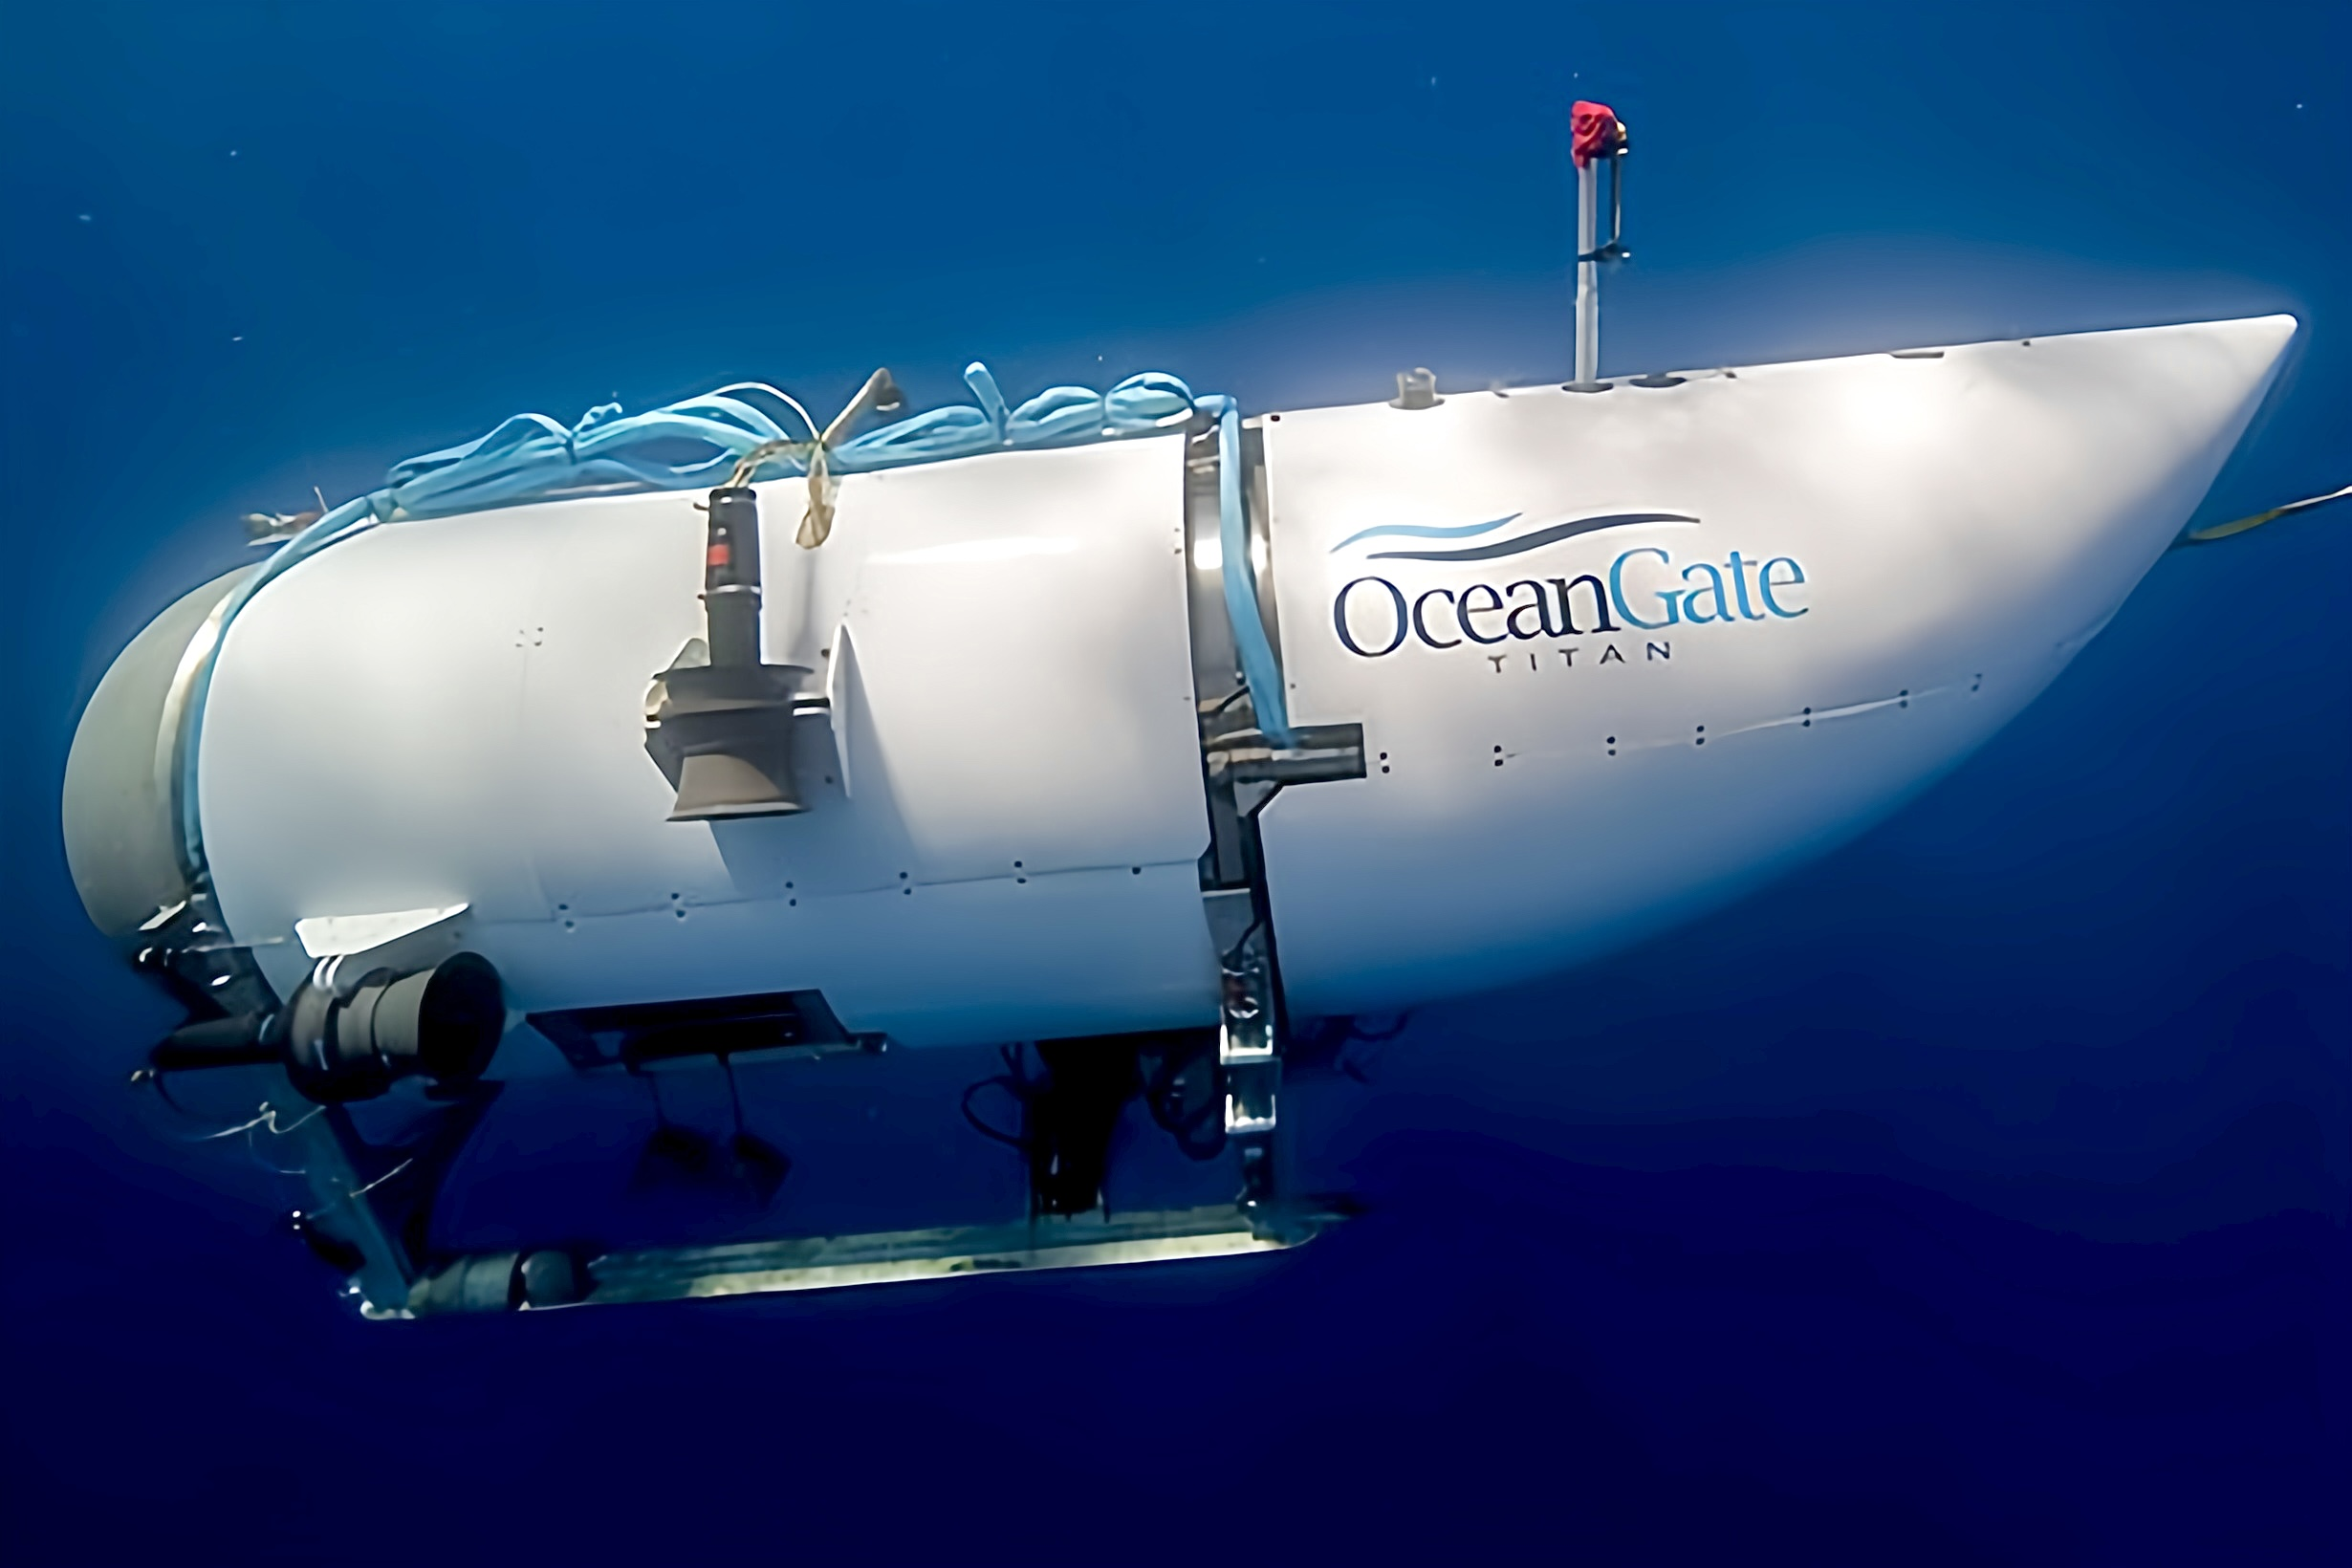
\includegraphics[width=7cm]{figure 1.jpg}  % 引入图片源
\caption{A picture of a submersible} \label{fig:A picture of a submersible}  % 标题与标签
\end{minipage}  % 子页结束
\hspace{0.02\textwidth}
\begin{minipage}[c]{0.48\textwidth}  % 子页
\centering  % 居中
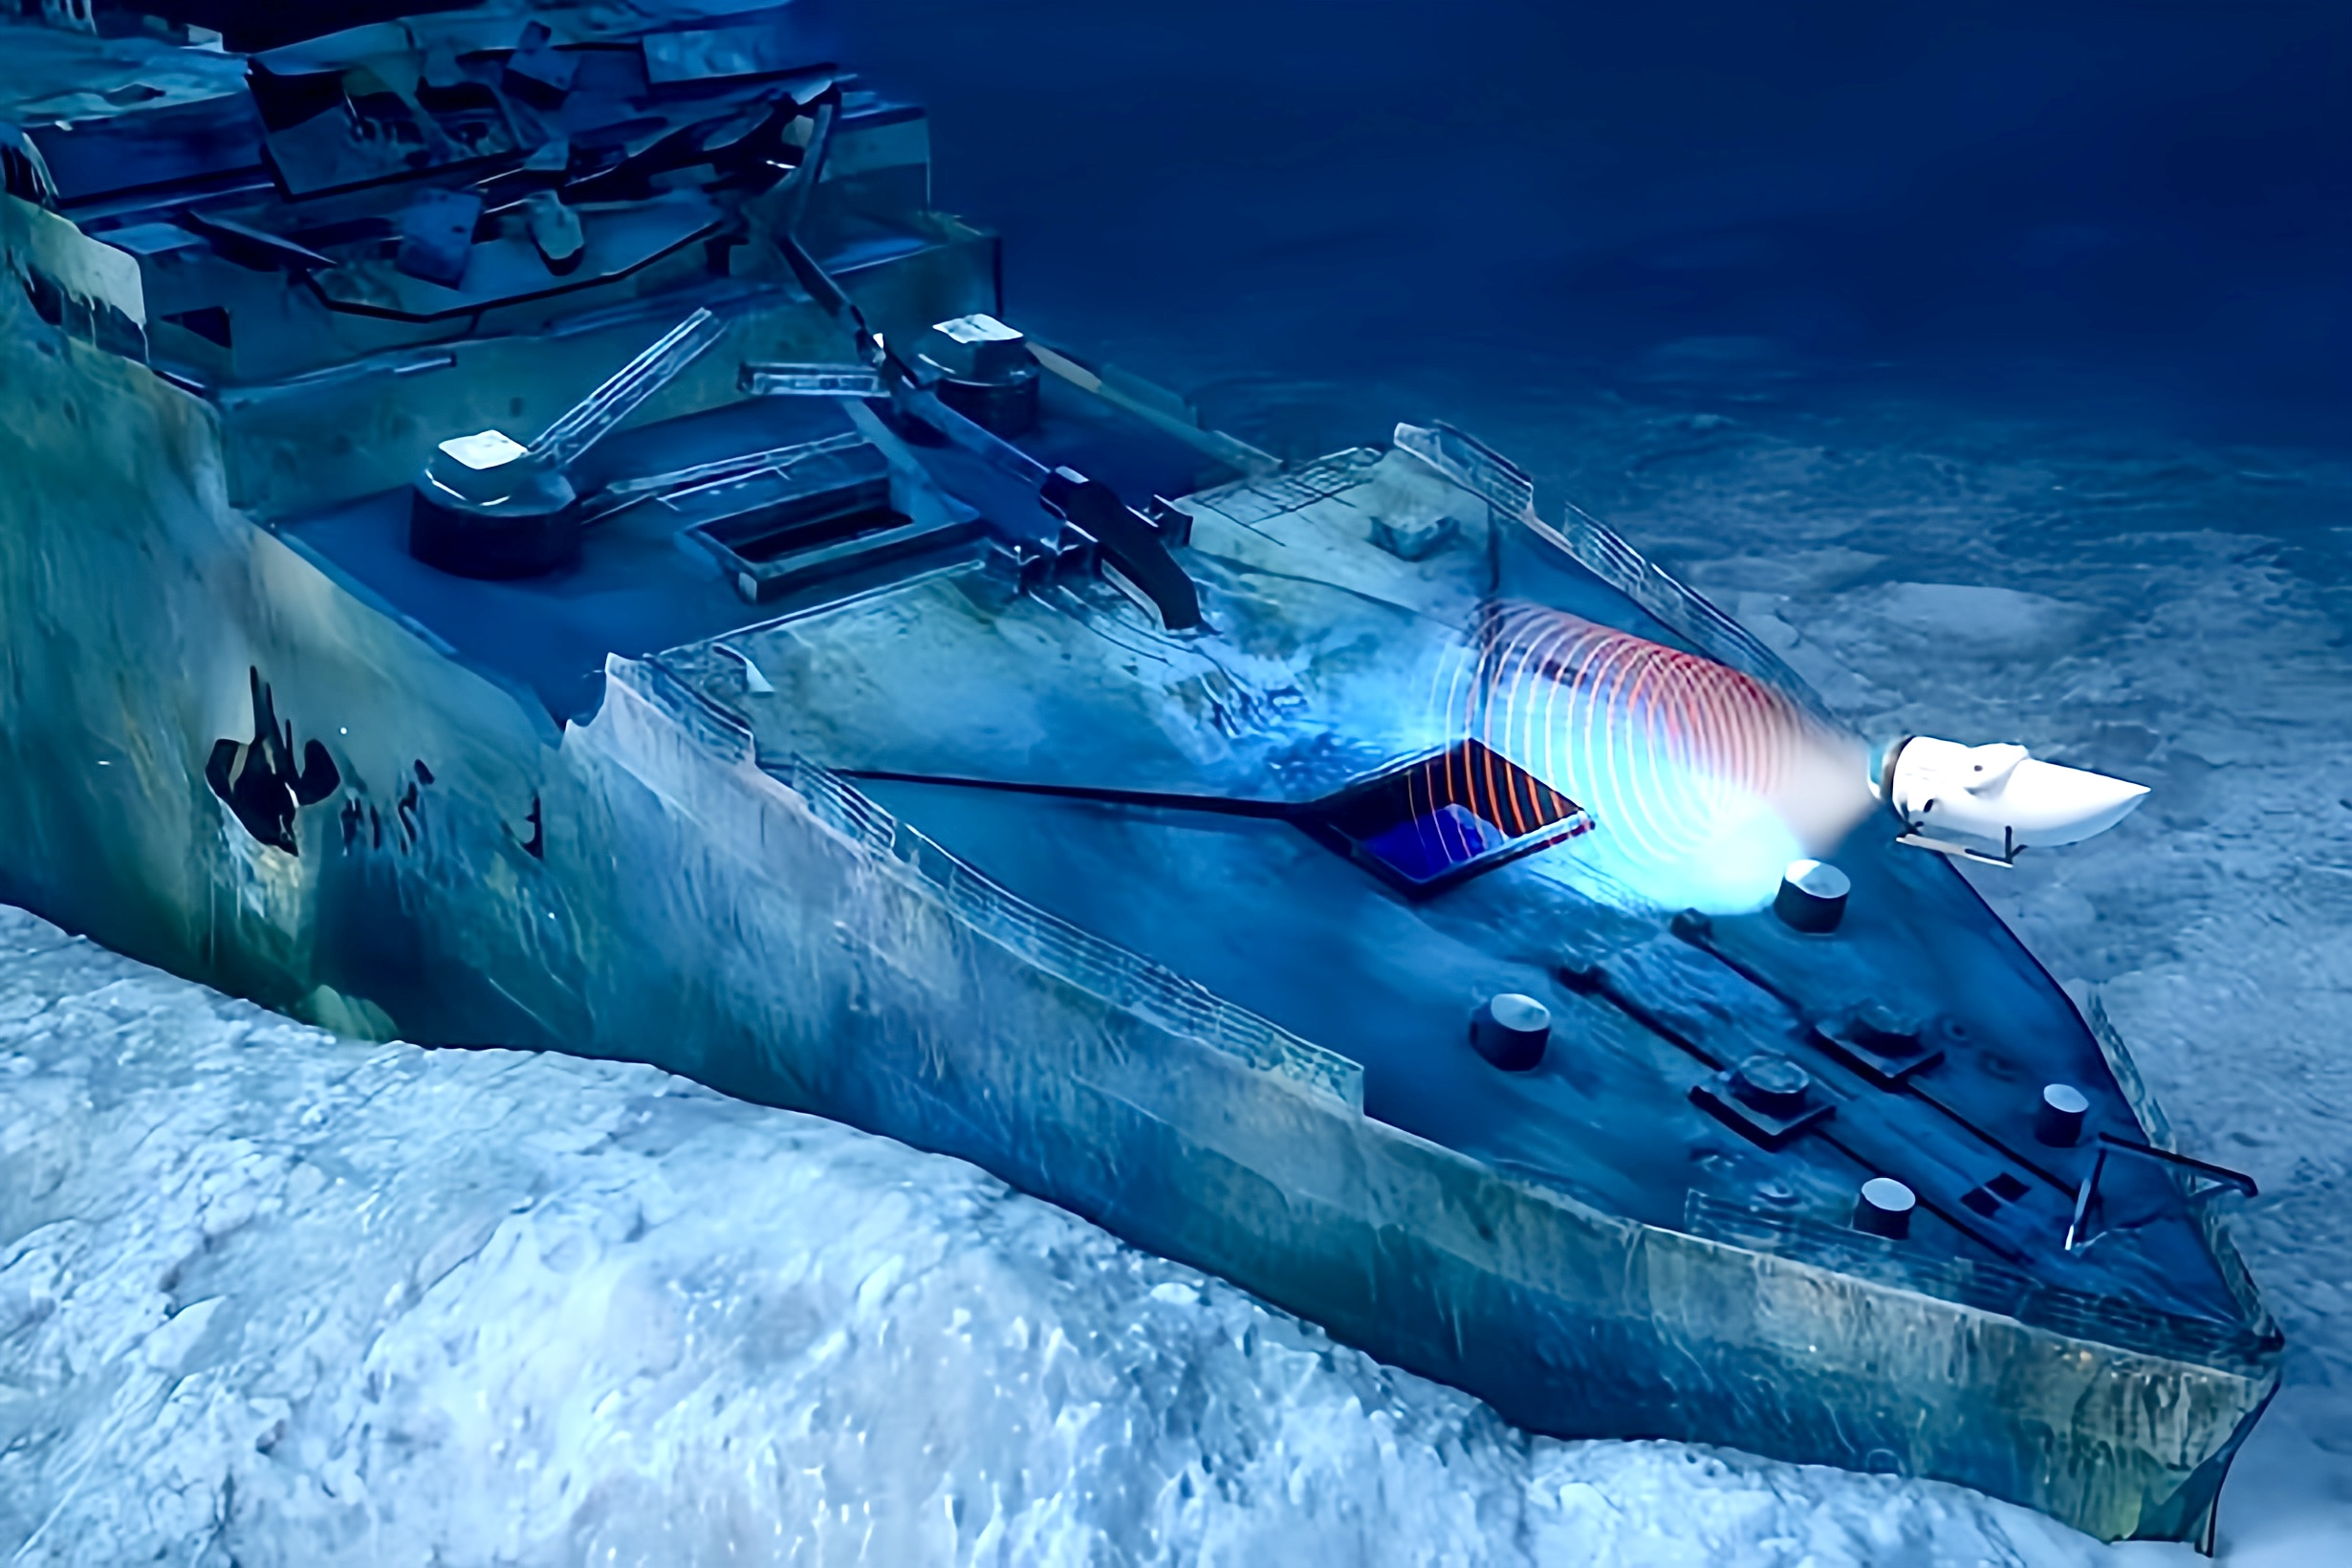
\includegraphics[width=7cm]{figure2.jpg}  % 引入图片源
\caption{Submersible explores the remains } \label{fig:The submersible explores the remains of the ship on the sea floor}  % 标题与标签
\end{minipage}  % 子页结束
\end{figure}  % 图片结束
%%%%%%%%%%%%%%%%%%%%%% 并排图结束 %%%%%%%%%%%%%%%%%%%%%%
%\begin{itemize}  % 无序列表
%\item This is a item.
%\item This is a item.
%\end{itemize}  % 无序列表结束
The loss of contact of the Titanic deep-sea submersible in 2023 caused an increase in the demand for submersible safety issues. The submersible oxygen reserve should be sufficient, the power system should be stable, and an effective backup system is also necessary \cite{Kirin}. The outside world needs to predict the position of the submersible over time and be able to find the missing submersible in the shortest possible time.
%\textit{I love math.}  % 斜体

%\textbf{I love math.}  % 粗体

%\underline{I love math.}  %下划线

\subsection{Restatement of the Problem}

Considering the background information and restricted conditions identified in the problem statement, we need to solve the following problems:
\begin{itemize}  % 无序列表

\item\textbf{Problem 1 }Build a model to predict the position of the submersible over time and account for uncertainties.


\item\textbf{Problem 2 }Advise the company on what search equipment to carry on the main ship and consider the availability, maintenance and cost of the equipment.

\item\textbf{Problem 3 }Build a model that uses the model information from question 1 to recommend equipment deployment patterns, the shortest time to find a missing submersible, and determine the probability of the submersible as a function of time and cumulative search results.

\item\textbf{Problem 4 }Consider how the model, extended to other tourist destinations such as the Caribbean, would need to change to account for multiple vehicles moving in the same region.
\end{itemize}  % 无序列表结束
\subsection{Literature Review}%补充文献综述部分


\subsection{Our Work}

\section{Assumptions and Justifications}

In order to solve the issues effectively,the following reasonable assumptions are formulated:
\begin{itemize}  % 无序列表

\item\textbf{Assumption 1 }
Seawater density is assumed to be linearly associated with depth.
\textbf{Justification :}\ \ Due to the differences in temperature and salinity, the phenomenon of vertical density stratification widely exists in the Marine environment. We can think that the submarine moves in this dense cline stratified by vertical density, and the density of the seawater, namely its depth, is linearly related.

\item\textbf{Assumption 2 }
Suppose that the submarine can be approximately regarded as a cylinder during the seabed movement.\\
\textbf{Justification : }
SUBOFF submarine model, as a scientific research submarine model, only has a few surface peripherals such as tail paddle. Compared with the size of the overall shape of the submarine, so SUBOFF can be regarded as the main body with only cylindrical submarine.
\item\textbf{Assumption 3 }
Assume that the surface of the submersible in contact with water is approximately smooth.\\
\textbf{Justification : }
Tourist submersibles have high safety performance requirements and are regularly maintained, with rare attachments or damages on their surface. Additionally, their surface is coated with a special material resistant to high pressure. According to Prandtl's theory of turbulent boundary layers, the surface of the submersible moving relative to the surrounding seawater can be considered approximately smooth. 
\item\textbf{Assumption 4 }
When extending the model to tourist destinations in the fourth question, all types of submarines for recreational diving must be deployed, and the main ship seeks to maximize profits while ensuring safety.\\
\textbf{Justification : }
 Based on ensuring safety, effective resource allocation, and optimizing operational strategies can enhance service efficiency and increase revenue. This assumption aligns with the fundamental principles and practical requirements of operating recreational facilities.
\end{itemize}  % 无序列表结束


\section{Notations}

%%%%%%%%%%%%%%%%%%%%%% 三线表开始 %%%%%%%%%%%%%%%%%%%%%%
\begin{table}[h]  % 表格
\caption{Notations used in this paper}  % 标题
\label{tab1}  % 标签
\tabcolsep 58pt % 列间距
\begin{tabular*}{\textwidth}{cccc}  % tabular*环境
\toprule  % 顶线
Symbol & Description & Unit  \\
\midrule  % 中线
Aaa & Bbb & Ccc \\
Aaa & Bbb & Ccc  \\
Aaa & Bbb & Ccc \\
\bottomrule  % 底线
\end{tabular*}  % tabular*环境结束
\end{table}  % 表格结束
%%%%%%%%%%%%%%%%%%%%%% 三线表结束 %%%%%%%%%%%%%%%%%%%%%%

\section{Model 1:Best search model  }% 一级标题
 

%\textit{Life Cycle Assessment (LCA)} is utilized as the primary methodology for this comprehensive analysis.  % 斜体

%\textbf{Environmental impacts} assessed in this study include global warming potential, acidification potential, and eutrophication potential.  % 粗体

%\underline{Sustainable strategies} for reducing the environmental impact of single-use plastics are proposed, based on the findings of the LCA.  % 下划线


\subsection{Preparation of the model}  % 二级标题
In our model, we need to consider the analysis of multiple modes of the submersible and its force situation, using some parameters of the submersible in the specific calculation, so we take the SUBOFF submarine model as the research object. Model parameters are as in Table 2 and the 3 D model is shown in Figure X.
\subsection{The Establishment of Model 1}
\subsubsection{analysis}
\subsubsection{guzhang}

\subsection{The Solution of Mod}
\subsubsection{xitong}
\subsubsection{qiantingxuanfu}
\subsubsection{zhangai}
\subsection{jiaozheng}
\section{zuiyou}
\subsection{zhuchuan}
\subsubsection{wentifenxi}
\subsubsection{zhunbei}
\subsubsection{qiujie}
\subsection{jiuyuan}
\subsubsection{fenxi}
\subsubsection{zhunebei}
\subsubsection{qiujie}
\section{zuidaunshijian}
\subsection{The Establishment of Model 3}
\subsubsection{GP-UCB}
\subsubsection{moxin}
\subsection{The Solution of Model 3}
\subsubsection{GP-UCB}
\subsubsection{tuihuo}






%%%%%%%%%%%%%%%%%%%%%%%% 并排图 %%%%%%%%%%%%%%%%%%%%%%%%

%%%%%%%%%%%%%%%%%%%%%% 并排图结束 %%%%%%%%%%%%%%%%%%%%%%

%%%%%%%%%%%%%%%%%%%%%%%% 三线表 %%%%%%%%%%%%%%%%%%%%%%%%




\section{Sensitivity Analysis}  % 一级标题

\section{Model Evaluation and Further Discussion}  % 一级标题

\section{Conclusion}  % 一级标题


\section{Analysis of the Problem}  % 一级标题

\begin{figure}[h]  % 图片
\small
\centering  % 居中
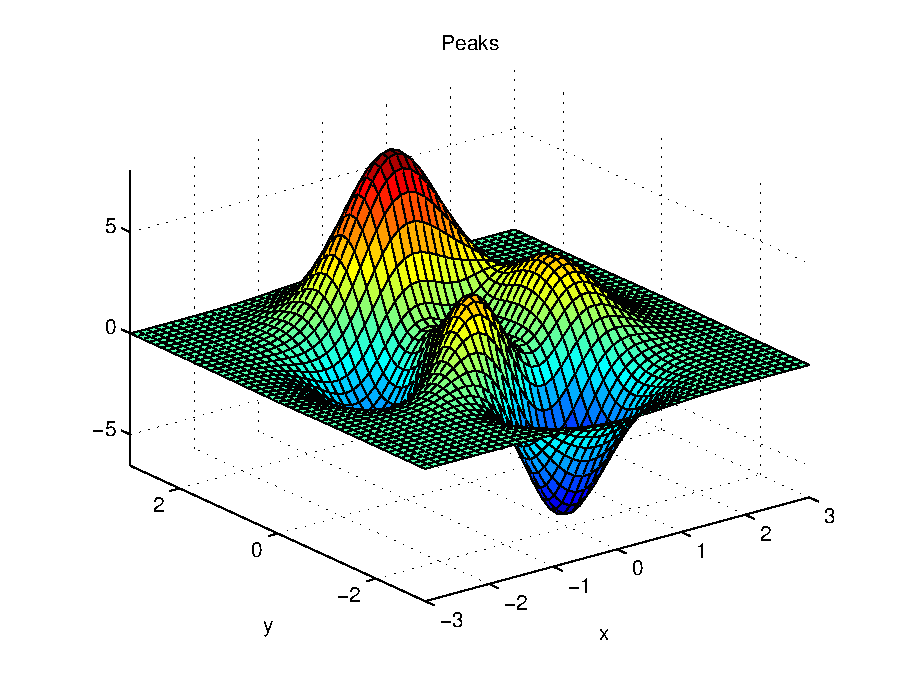
\includegraphics[width=12cm]{example.eps}  % 引入图片源
\caption{example} \label{fig:example}  % 标题与标签
\end{figure}  % 图片结束

This is Figure \eqref{fig:example}.  % 引用图表

This is a cite\cite{vaswani2017attention}.  % 引用文献

\begin{equation}  % 公式,独占一行、居中,自动编号
E = mc^2 \label{aa}  % 标签
\end{equation}  % 公式结束

\begin{equation}  % 公式,独占一行、居中
\nonumber % 不编号
E = mc^2
\end{equation}  % 公式结束

\printbibliography  % 打印引用文献列表

%%%%%%%%%%%%%%%%%%%%%%% 正文结束 %%%%%%%%%%%%%%%%%%%%%%%

\begin{appendices}  % 附录

\begin{memo}[Memorandum]  % 建议书
	This is a memorandum.
\end{memo}  % 建议书结束

\section{First appendix}  % 一级标题

Here are simulation programmes we used in our model as follow.\\
\textbf{MATLAB source code:}
\lstinputlisting[language=Matlab]{./code/matlab.m}

\section{Second appendix}  % 一级标题

\textbf{Python source code:}
\lstinputlisting[language=C++]{./code/python.py}

\end{appendices}  % 附录结束
\end{document}  % 文档结束
%%%%%%%%%%%%%%%%%%%%%%%%%%%%%%%%%%%%%%%%%%%%%%%%%%%%%%%